\section{Introduction}

Execution traces record a program's complete runtime behavior: every function call, variable assignment, and control flow decision.
Recent work has incorporated them into code language models for tasks from bug localization to program repair \citep{chen2025tracepile,ding2024traced,wang2025dcsh,ni2024next}, under the working assumption that richer runtime information yields better predictions.
\emph{We find the opposite.}
For verdict prediction (classifying whether a test passes or fails), feeding a model the complete execution trace produces accuracies of 79--82\%, barely above a source-code-only baseline (72--76\%), while a single compact component of the same trace reaches ${\geq}$99.33\% across all models tested.
Verbose traces do not just fail to help; they actively impair learning.

Verdict prediction offers a clean testbed for isolating this effect.
As binary classification, it separates signal extraction from generation noise; as fault detection, the model need only detect failure, not simulate execution.
If the fault signal concentrates in a small trace subset, information density should matter more than quantity.
Prior work found no single trace representation consistently outperforms others \citep{wang2025dcsh}, but focused on generation tasks where this density hypothesis could not be cleanly tested.

We conduct the first systematic component ablation of trace representations, decomposing Verdict-Optimized Trace Abstraction (VOTA; exception events + assertion comparisons + loop compression) into individual components across four models spanning 1.5B to 13B parameters and three architecture families \citep{qwen2025coder,roziere2024code,deepseek2024coder}, on 591 problems from HumanEval \citep{chen2021evaluating} and MBPP-sanitized \citep{austin2021program}.
The results are unambiguous: exception events (a median of 150 tokens encoding error type, stack frame, and message) reach ${\geq}$99.33\% accuracy across all models and seeds, converging within 50 training steps.
Full traces plateau near 82\% and gradient-masked variants reach only ${\sim}$86\%, both without stable convergence. This confirms that information density, not model capacity, is the binding constraint (Figure~\ref{fig:training_dynamics}).

This finding is robust to several potential confounds.
Removing format markers preserves accuracy within 2pp, and on 8 boundary samples where exceptions appear in passing code, the fine-tuned model correctly classifies 6/8 vs.\ 0/8 for a regex baseline, which confirms the signal is semantic (\S\ref{sec:nomarker}).
Gradient masking bounds the backward-pass contribution to ${\sim}$4pp (\S\ref{sec:density}), a tail-truncation budget sweep across four models reveals a phase transition at ${\sim}$500 tokens (\S\ref{sec:trace_length}), and cross-dataset transfer to DebugBench ($N{=}426$) preserves the component ranking (\S\ref{sec:debugbench}).

Our contributions:
\begin{enumerate}
\item \textbf{Information density as the binding constraint on supervised fine-tuning (SFT) learning}: training dynamics, gradient masking (${\sim}$4pp backward-pass contribution), and cross-model convergence confirm that compact trace inputs learn faster and more stably than verbose ones, independent of model scale (\S\ref{sec:ablation}, \S\ref{sec:density}).
\item \textbf{Exception events as the minimal sufficient signal}: ${\geq}$99.33\% across all four models with zero cross-seed variance on Qwen and sub-1pp cross-model range (\S\ref{sec:cross_model}).
\item \textbf{A two-tier diagnostic hierarchy with quantitative decomposition}: Tier~1 signals (exceptions, assertion comparisons) are individually sufficient for near-perfect accuracy and generalize across architectures within a 0.50--1.11pp cross-model range, while Tier~2 signals (loop compression) are model-dependent with ${\sim}$9pp range; a sharp phase transition at ${\sim}$500 tail tokens spatially localizes the diagnostic boundary (\S\ref{sec:ablation}, \S\ref{sec:trace_length}).
\end{enumerate}

\begin{figure}[t]
\centering
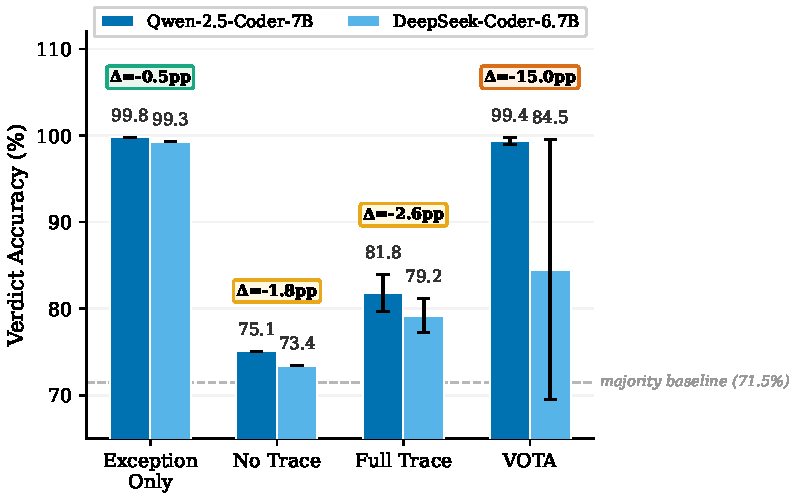
\includegraphics[width=\columnwidth]{fig3_cross_model_gap}
\caption{Cross-model verdict accuracy by trace condition (Qwen-2.5-Coder-7B vs.\ DeepSeek-Coder-6.7B, $N{=}1{,}190$). \cond{exception\_only} shows near-identical accuracy across models ($\Delta{=}0.5$pp), while \cond{VOTA} exhibits a 15pp cross-model gap due to a tokenizer-induced training failure (Appendix~\ref{sec:tokenizer_analysis}).}
\label{fig:cross_scale}
\end{figure}
